\documentclass{beamer}

\usetheme{Madrid}
\usepackage{graphicx}

\title[SKBD] {SKBD: Segment Knotting Boundary Detection For Room Layout Detection}

\author[Pictures]
{Barna Mikler \and Botond Geonczeol \and Dominik Li \and \\ Matyas David \and Balint Boros}

\institute[ELTE]{Eötvös Loránd University \\ Faculty of Informatics}

\date[2024] {November 2024}

\logo{
\includegraphics[height=1cm]{images/elte_cimer_szines.eps}}

\begin{document}

\frame{\titlepage}

\begin{frame}
\frametitle{Table of Contents}
\tableofcontents
\end{frame}  

\section{Motivation}
\begin{frame}
\frametitle{Motivation}
\begin{itemize}
    \item Manhattan World Assumption or cuboid shapes.
    \item Meeting the growing demand for flexible and accurate room layout reconstruction in applications
    \item Automating the floor plan generation process to replace labor-intensive and error-prone manual techniques.
    \item Enhancing robustness to occlusions, clutter, and diverse viewpoints for better performance in challenging environments.
    \item Advancing state-of-the-art methods by introducing SKBD
\end{itemize}

\end{frame}

\section{Reconstruction of Non-Cuboid Spaces}
\begin{frame}
\frametitle{Reconstruction of Non-Cuboid Spaces}
\begin{itemize}
\item Existing reconstruction methods assume cuboid shapes, which don’t work for rooms with irregular shapes, such as curved walls or slanted ceilings.
\item Non-cuboid rooms have complex geometries that make accurate reconstruction difficult, especially when working with limited or single-image inputs.
\item A method that can reconstruct room layouts of any shape, including non-cuboid spaces, by improving upon traditional approaches.
\item SKBD connects segments in images to detect relationships between parts of the room, improving accuracy by using multiple images and detecting connections beyond simple proximity.
\end{itemize}
\end{frame}

\section{Terminology}
\begin{frame}
\frametitle{Terminology}

\begin{itemize}
    \item Global descriptor: represents features of the entire image. E.g.: color histograms, texture descriptors, edge histograms
    \item Local descriptor: represents features of specific points or regions of the image. E.g.: SIFT (Scale-Invariant Feature Transform), SURF (Speeded-Up Robust Features)
    \item Semantic segment: A distinct part of the image that specifies individual objects or an important region
    \item Representation: A descriptor detailing a segment
    \item Knot: A group of segments collected around a key point that are similar
\end{itemize}

%Knot - Later probably
%Super segment - Later probably
%Floor map - Can be possibly skipped
\end{frame}

% Skip some of the methodology or merge frames maybe
% I think they are important, but it might be too long
\section{Detection of Distinct Segments}
\begin{frame}
\frametitle{Detection of Distinct Segments}

\begin{itemize}
    \item Local Descriptors
    \item Reduction of found representations through a grouping algorithm
    \item Confidence level for segments in the set
\end{itemize}

\end{frame}

\begin{frame}
\frametitle{Detection of Distinct Segments}

\begin{figure}[htbp]
    \centering
    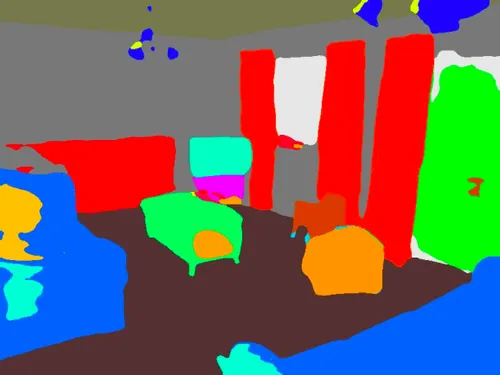
\includegraphics[width=0.5\textwidth]{images/objdet.png}
    \caption{Detecting objects using descriptors}
    \label{fig:desc_objdet}
\end{figure}

\end{frame}

\begin{frame}
\frametitle{Detection of Distinct Segments}

\begin{figure}[htbp]
    \centering
    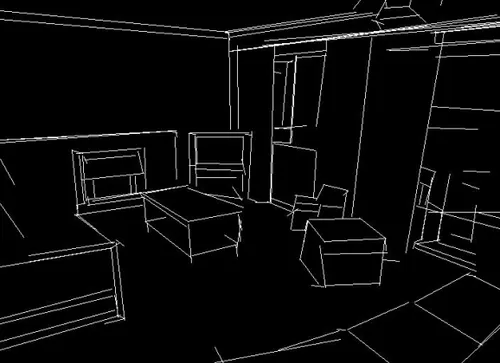
\includegraphics[width=0.5\textwidth]{images/edgedet.png}
    \caption{Detecting edges using descriptors}
    \label{fig:desc_objdet}
\end{figure}

\end{frame}

\begin{frame}
\frametitle{Detection of Distinct Segments}
\textbf{Key Steps:}
    \begin{itemize}
        \item Extract representations \( R = \{r_1, r_2, \dots, r_n\} \).
        \item Initialize segment set \(S=\{\}\)
        \item Compare representations:
        \[
        \text{Sim}(r_j,s_i) \geq \tau \implies \text{keep } s_i \text{ as main} \; (i = 0 \dots \lvert S \lvert, j=0\dots \lvert R \lvert)
         \]
         \[
         \text{Sim}(r_j, r_l) \geq \tau \implies \text{group together, add to S} \; (l=0\dots \lvert R \lvert)
         \]
        \item Assign confidence:
        \[
        C(s_i) \propto \text{Number of supporting representations.}
        \]
        \item Output distinct segments \( S = \{s_1, s_2, \dots, s_m\} \) with confidence levels.
    \end{itemize}
\end{frame}


\section{Association of Segments}
\begin{frame}
\frametitle{Association of Segments}
\begin{itemize}
    \item Calculating interest score for each segments
    \item Choosing segments with the highest score as key points
    \item Associating segments with key points based on association score, forming knots
    \item Repeat until there are enough knots
\end{itemize}
\end{frame}

\section{Connection of Knots}
\begin{frame}
\frametitle{Connection of Knots}
\begin{itemize}
    \item Determining a super segment for each knot
    \item Calculating connection strength between each super segment, creating the CSSM
    \item Normalizing values in rows
\end{itemize}
\end{frame}

\section{Layout Guess and Reconstruction}
\begin{frame}
\frametitle{Layout Guess and Reconstruction}
\begin{itemize}
    \item Building graph guesses
    \item Selecting the main layout
    \item Reconstructing the floormap
\end{itemize}
\end{frame}

\begin{frame}
\frametitle{Layout Guess and Reconstruction}

    \begin{itemize}
    \item Creating CSSM on a subset of characteristics
    \item Proximity values \( p_i \) selected from a range defined by quartiles:
    \[
     p_i \in [Q_1(\text{CSSM}), Q_3(\text{CSSM})] \; \forall i=1\dots k
    \]
    
    \item Let \( G_i \) be the \( i \)-th graph, where the nodes are depictions \( V(G_i) \) and the edges are \( E(G_i) \).
    \item Weight of an edge \( e_{ij} \in E(G_i) \), given by the CSSM strength score:
    \[
    w(e_{ij})_{i\ne j} = \text{CSSM}(r_i, r_j)
    \]
    \item An edge is formed between two depictions \( r_i \) and \( r_j \) if:
    \[
    \text{CSSM}(r_i, r_j) \geq p_i
    \]
    
\end{itemize}
\end{frame}

\begin{frame}
\frametitle{Layout Guess and Reconstruction}
\textbf{The final floor map contains:}
\begin{itemize}
    \item Points for every corner
    \item Data about the distance between these corners
    \item Special flags for door or window corners
    \item information about room height when possible
\end{itemize}
\end{frame}


\section{Overall Results}
\begin{frame}
\frametitle{Overall Results}
Results
\end{frame}

\section{Results on Structured3D and LSUN}
\begin{frame}
\frametitle{Results on Structured3D and LSUN}
Results
\end{frame}

% Split or give more frames?
\section{Discussion}
\begin{frame}
\frametitle{Discussion}
Discussion
\end{frame}

\section{Conclusion}
\begin{frame}
\frametitle{Conclusion}
\textbf{Goal of the paper:}
\begin{itemize}
    \item Reconstruct a room's floormap
    \item Use as few images as possible
    \item Present floormap as an easily processable data-structure
\end{itemize}
\textbf{Obtained results:}
\begin{itemize}
    \item Solution outperforms existing methods on multiple databases.
    \item Delivers a highly usable output that is easy to process.
\end{itemize}
\textbf{Achieved impact:}
\begin{itemize}
    \item Enables the development of various services and applications.
    \item Efficient and accurate spatial mapping for future use.
\end{itemize}
\end{frame}

\section{Future Work}
\begin{frame}
\frametitle{Future Work}
\begin{itemize}
    \item Exploring advanced descriptors (e.g. DALSM), potentially improving benchmark results.
    \item Incorporating multi-view stereo or Structure-from-Motion (SfM) techniques to achieve (CE) rates below 0.5\%.
    \item Expanding SKBD’s robustness against varying image qualities and environmental conditions. 
    \item Optimize SKBD for simpler cuboid room layouts without sacrificing its generalizability to non-cuboid spaces.
    \item Reducing computational complexity of the CSSM generation process.
    \item Testing SKBD on diverse real-world datasets.
\end{itemize}
\end{frame}

% We could skip this, kinda useless, but the names are kinda funny
\section{Acknowledgments}
\begin{frame}
\frametitle{Acknowledgments}
Special thanks to
\begin{itemize}
    \item European Union's Horizon Europe Research and Innovation Programme
    \item Dr. Philip Miner
    \item Dr. Keve Tevesy
\end{itemize}
\end{frame}

\section{Q\&A}
\begin{frame}
\frametitle{Q\&A}
Q\&A
\end{frame}

\end{document}
